\subsection{Behavior}
\label{sec:setup.quad.hybrid.behavior}

\Cref{fig:setup.quad.hybrid.period} shows the 2D scans of the periods of the stable cycles of the model.
As before, \Cref{fig:setup.quad.hybrid.period.halved} shows the adjusted model to indicate ``type B'' parameter regions.
The structure did not change much.
There are still chains of parameter regions with the same period next to each other.
With each chain alternating between ``type A'' and ``type B'' parameter regions.
Now the ``type B'' parameter regions are even more prominent in the chains for larger values of $\beta$.
This was not the case in the fully piecewise quadratic model in \Cref{sec:setup.quad.hyper.2}.

\begin{figure}
	\centering
	\begin{subfigure}{0.4\textwidth}
		\centering
		\includegraphics[width=\textwidth]{50_Quadratic_linearR/2D_Period_Whole/result.png}
		\caption{Normal model}
		\label{fig:setup.quad.hybrid.period.full}
	\end{subfigure}
	\begin{subfigure}{0.4\textwidth}
		\centering
		\includegraphics[width=\textwidth]{51_Quadratic_linearR_Halved/2D_Period_Whole/result.png}
		\caption{Adjusted model}
		\label{fig:setup.quad.hybrid.period.halved}
	\end{subfigure}
	\caption[2D scan of the periods of the piecewise hybrid quadratic model with hyperparameters]{
		2D scan of the periods of the piecewise hybrid quadratic model with hyperparameters $g_R\left(\frac{1}{4}\right)$ and $g_R\left(\frac{1}{2}\right)$.
		The parameters $a_L = 4, b_L = -\frac{1}{2},$ and $g_R\left(\frac{1}{4}\right) = 0.525$ are fixed.
		The parameters $\alpha = -g_R\left(\frac{1}{4}\right)$ and $\beta = c_L$ are varied in the ranges $[-0.45, -0.275]$ and $[0.15, 0.1875]$, respectively.
		The points $A, B,$ and $C$ mark the parameter values used for the cobweb diagrams in \Cref{fig:setup.quad.hybrid.cobwebs}.
		(a) shows the scan for the normal model as defined above, while (b) shows the scan for the adjusted model where we can see ``type B'' parameter regions as they have higher periods in the adjusted model.
	}
	\label{fig:setup.quad.hybrid.period}
\end{figure}

\begin{figure}
	\centering
	\begin{subfigure}{0.3\textwidth}
		\centering
		\includegraphics[width=\textwidth]{50_Quadratic_linearR/Cobweb_A/result.png}
		\caption{At point $A$}
		\label{fig:setup.quad.hybrid.cobweb.A}
	\end{subfigure}
	\begin{subfigure}{0.3\textwidth}
		\centering
		\includegraphics[width=\textwidth]{50_Quadratic_linearR/Cobweb_B/result.png}
		\caption{At point $B$}
		\label{fig:setup.quad.hybrid.cobweb.B}
	\end{subfigure}
	\begin{subfigure}{0.3\textwidth}
		\centering
		\includegraphics[width=\textwidth]{50_Quadratic_linearR/Cobweb_C/result.png}
		\caption{At point $C$}
		\label{fig:setup.quad.hybrid.cobweb.C}
	\end{subfigure}
	\caption[Cobwebs of the piecewise hybrid quadratic model with hyperparameters]{
		Cobweb diagrams at three parameter values of $\alpha = -g_R\left(\frac{1}{4}\right)$ and $\beta = c_L$ in the piecewise hybrid quadratic model with hyperparameters.
		The other parameters are fixed as $a_L = 4, b_L = -\frac{1}{2},$ and $g_R\left(\frac{1}{2}\right) = \frac{1}{2} + \frac{1}{40}$.
		The parameter values are marked in \Cref{fig:setup.quad.hybrid.period}.
	}
	\label{fig:setup.quad.hybrid.cobwebs}
\end{figure}

Looking at the cobweb diagrams of the stable cycles at the points marked in \Cref{fig:setup.quad.hybrid.period} confirms that we still have the same behavior as in \Cref{sec:setup.quad.hyper.2}.
All stable cycles in the chain are of period 18.
The symbolic sequence of the stable cycle at point $A$ is $\A^6\B^3\C^6\D^3$.
At point $C$, the symbolic sequence of the stable cycle is $\A^5\B^4\C^5\D^4$.
And in between, at point $C$ there are 2 coexisting cycles with symbolic sequences $\A^6\B^3\C^5\D^4$ and $\A^5\B^4\C^6\D^3$, respectively.
As described in \Cref{sec:setup.quad.hyper.2}, this is exactly like the original model behaves.

\Cref{fig:setup.quad.hybrid.og} shows the 2D period scans of the original model again.
This time also with an adjusted version of the original model that allows to see the ``type B'' parameter regions.
The scans of the original model and the hybrid piecewise quadratic model defined in this section look alike.
Therefore, we will now refer to the hybrid piecewise quadratic model defined here as the archetypal model for the bifurcation structures observed in the original model.

\begin{figure}
	\centering
	\begin{subfigure}{0.4\textwidth}
		\centering
		\includegraphics[width=\textwidth]{99_Yunus/2D_Period_Zoomed_noPoints/result.png}
		\caption{Normal Model}
		\label{fig:setup.quad.hybrid.og.halved.full}
	\end{subfigure}
	\begin{subfigure}{0.4\textwidth}
		\centering
		\includegraphics[width=\textwidth]{98_Yunus_modpi/2D_Period_Zoomed_noPoints/result.png}
		\caption{Adjusted Model}
		\label{fig:setup.quad.hybrid.og.halved}
	\end{subfigure}
	\caption[2D scan of the periods of the original model for comparison]{
		2D scan of the periods of the original model for comparison with \Cref{fig:setup.quad.hybrid.period}, the 2D scan of the periods of the piecewise hybrid quadratic model.
		(a) shows the scan for the normal model, while (b) shows the scan for the adjusted model where we can see ``type B'' parameter regions as they have higher periods in the adjusted model.
	}
	\label{fig:setup.quad.hybrid.og}
\end{figure}
